\input{commun/presentations.tex}
\def\siecle#1{\textsc{\romannumeral #1}\textsuperscript{e}~siècle}

\title[Séance 11 - Histoire]{Séance 11 \\ Histoire}

\begin{document}
 \begin{frame}
 \titlepage
 \end{frame}
 
 \begin{frame}
 \tableofcontents
 \end{frame}
 
 \section{Un rêve humain intemporel : voler}
 	\subsection{Mythologie puis les premiers ingénieurs}
	\begin{frame}{Un rêve humain intemporel : voler}
	\begin{columns}
		\begin{column}{0.4\textwidth}
		\begin{figure}[H]
			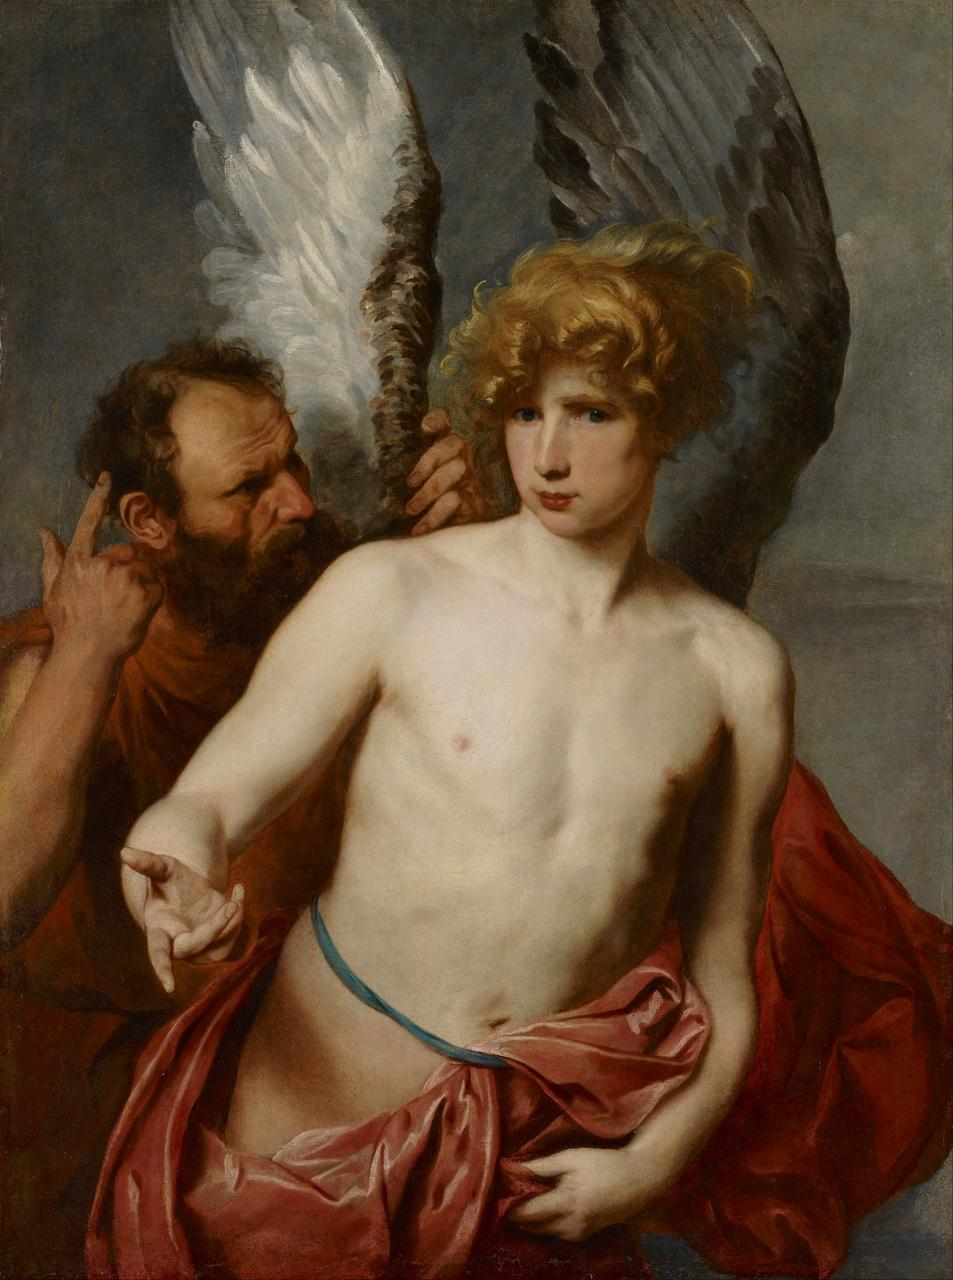
\includegraphics[width=0.9\linewidth]{Annexes/friseChronologique/img/Anthony_van_Dyck_-_Daedalus_and_Icarus_-_Google_Art_Project.jpg}
			\legende{Icare et Dédale}{frise:Anthony_van_Dyck_-_Daedalus_and_Icarus_-_Google_Art_Project.jpg}
		\end{figure}	
		\end{column}
		\begin{column}{0.6\textwidth}
			Le mythe d'Icare (800 av JC) illustre que l'homme à toujours rêver de voler. \newline
		
			Dans la mythologie grecque, Dédale fabrique des ailes en plumes et en cire pour lui et son fils Icare afin de s'échapper du labyrinthe. Icare, s'approchant trop près du soleil, voit la cire fondre et tombe dans la mer. Ce mythe illustre depuis l'Antiquité le rêve ancestral de l'Homme de voler.
		\end{column}
		\end{columns}
	\end{frame} 	
	
	\begin{frame}{Leonard de Vinci : ingénieur visionnaire}
	\begin{columns}
		\begin{column}{0.4\textwidth}
		\begin{figure}[H]
			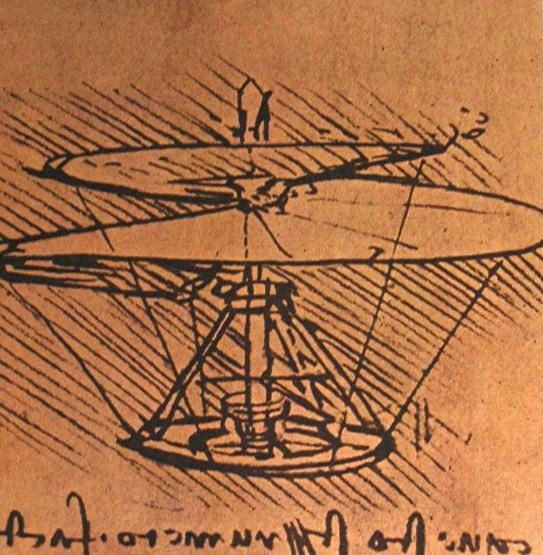
\includegraphics[width=1.0\linewidth]{Annexes/friseChronologique/img/Leonardo_helicopter.JPG}
			\legende{Étude de la vis aérienne de Léonard de Vinci}{frise:Leonardo_helicopter.JPG}
		\end{figure}	
		\end{column}
		\begin{column}{0.6\textwidth}
			Léonard de Vinci étudie le vol des oiseaux et conçoit de nombreuses machines volantes dans ses carnets : l'ornithoptère (machine à ailes battantes), le parachute pyramidal, et une vis aérienne (ancêtre de l'hélicoptère). Bien que jamais construites de son vivant, ses études pionnières influenceront les inventeurs futurs.
		\end{column}
		\end{columns}
	\end{frame} 	
	
	\subsection{L'ère des plus légers que l'air}
	\begin{frame}{Plus léger que l'air : la montgolfière}
	\begin{columns}
		\begin{column}{0.4\textwidth}
		\begin{figure}[H]
			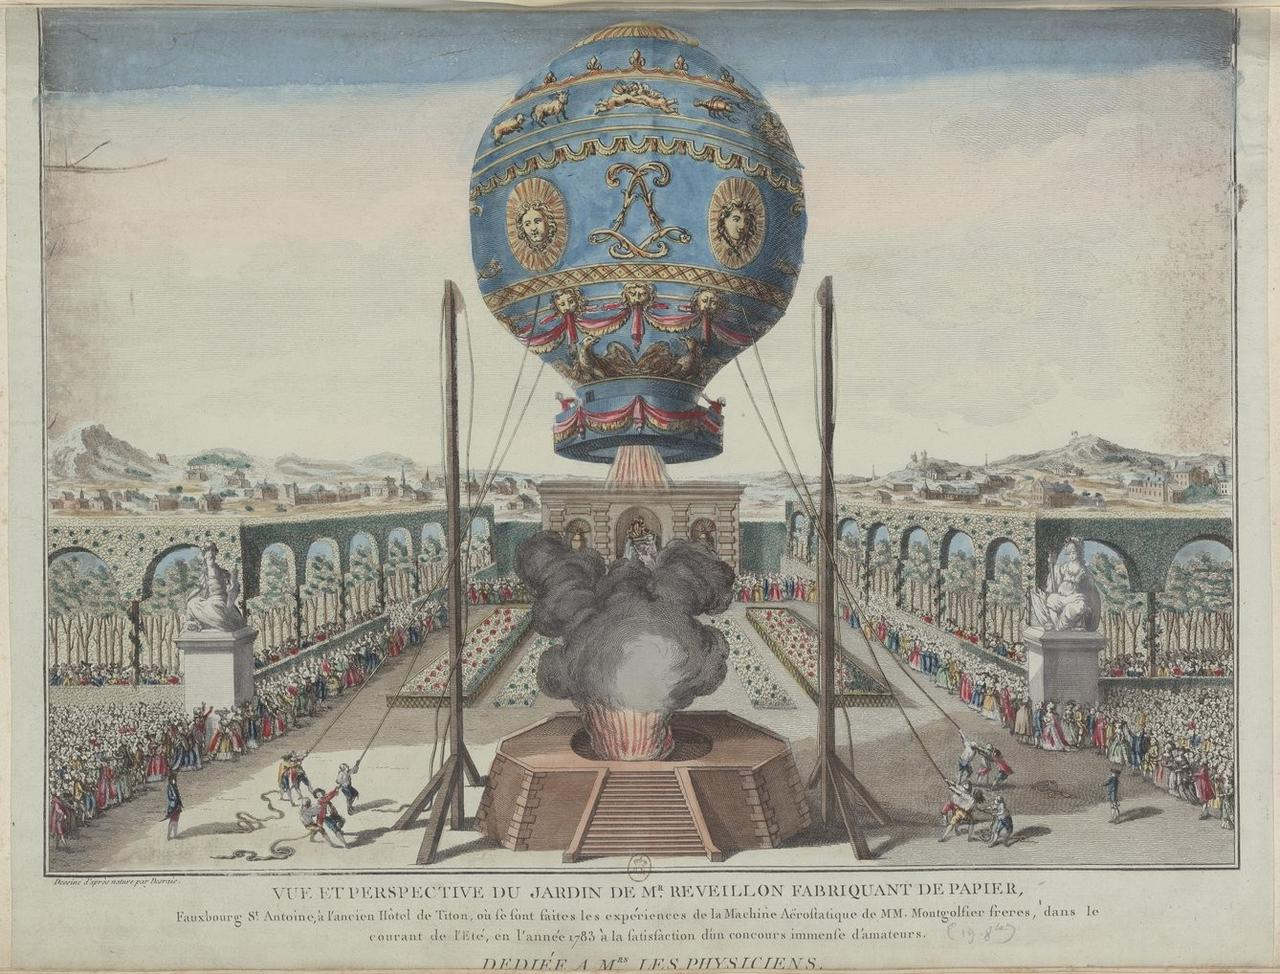
\includegraphics[width=1.0\linewidth]{Annexes/friseChronologique/img/Montgolfiere_1783.jpg}
			\legende{Ascension captive d'une montgolfière (Jean-François Pilâtre de Rozier) dans les jardins de la papèterie Réveillon, le 19 octobre 1783.}{frise:Montgolfiere_1783.jpg}
		\end{figure}	
		\end{column}
		\begin{column}{0.6\textwidth}
			A la fin du \siecle{18} nait l'aérostation : c'est l'ensemble des techniques visant à utiliser les gaz plus légers que l'air pour s'élever dans les airs. \newline
			
			Le 19 septembre 1783, à Paris, les frères Montgolfier font voler pour la première fois des êtres vivants : un coq, un canard et un mouton. \newline
			
			Le 21 novembre 1783, ils renouvellent l'expérience, avec à bord, Pilâtre de Rosier, qui devient donc le premier humain à voler.
			
			
		\end{column}
		\end{columns}
	\end{frame} 	
	
	\begin{frame}{Plus léger que l'air : le ballon à gaz}
	\begin{columns}
		\begin{column}{0.4\textwidth}
		\begin{figure}[H]
			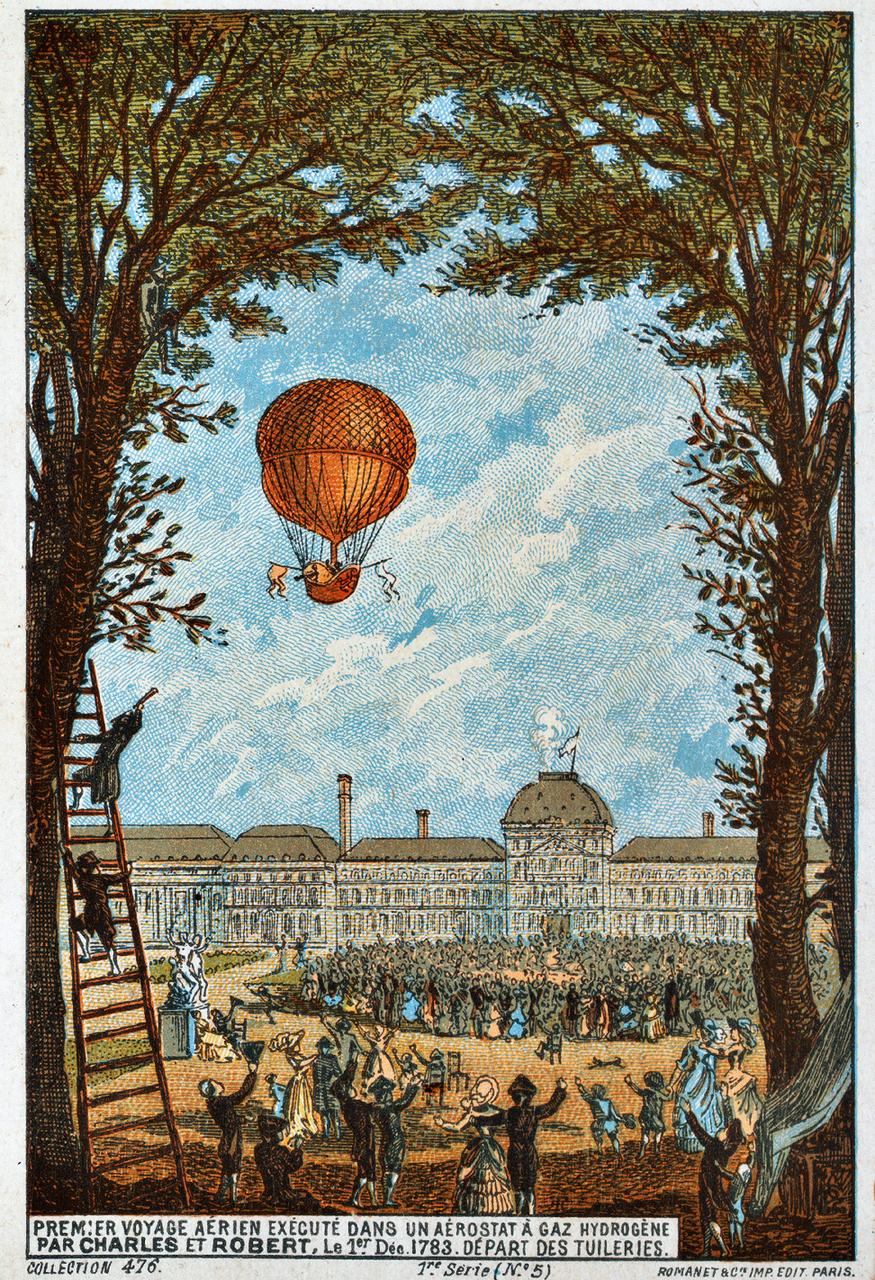
\includegraphics[width=0.8\linewidth]{Annexes/friseChronologique/img/Early_flight_02562u_28529.jpg}
			\legende{Ballon à gaz de Jacques Charles}{frise:Early_flight_02562u_28529.jpg}
		\end{figure}	
		\end{column}
		\begin{column}{0.6\textwidth}
			Le 1er décembre 1783, l'inventeur français Jacques Charles effectue le premier vol en ballon à gaz, gonflé à l'hydrogène. Ce type de ballon permet des vols plus longs et plus hauts que les ballons à air chaud. \newline
			
			Le 7 janvier 1785, Jean-Pierre Blanchard traverse la Manche en ballon à hydrogène. Il s'agit de la première traversée de la Manche avec un aéronef, 124 avant celle de Louis Blériot.	
		\end{column}
		\end{columns}
	\end{frame} 	
	
	\begin{frame}{Plus léger que l'air : le dirigeable}
	\begin{columns}
		\begin{column}{0.4\textwidth}
		\begin{figure}[H]
			
\includegraphics[width=0.8\linewidth]{Annexes/friseChronologique/extraitsVideo/premierVolDirigeable.png}
			\legende{Le dirigeable de Henri Giffard}{frise:premierVolDirigeable.png}
		\end{figure}	
		\end{column}
		\begin{column}{0.6\textwidth}
			Le 24 septembre 1852 l'ingénieur français Henri Giffard fait voler le premier dirigeable, propulsé par un moteur à vapeur.
			
			
		\end{column}
		\end{columns}
	\end{frame} 
	
	\section{Plus lourds que l'air}
		\subsection{Les pionniers}	
	\begin{frame}{Premiers pas des plus lourds que l'air}
	\begin{columns}
		\begin{column}{0.4\textwidth}
		\begin{figure}[H]
			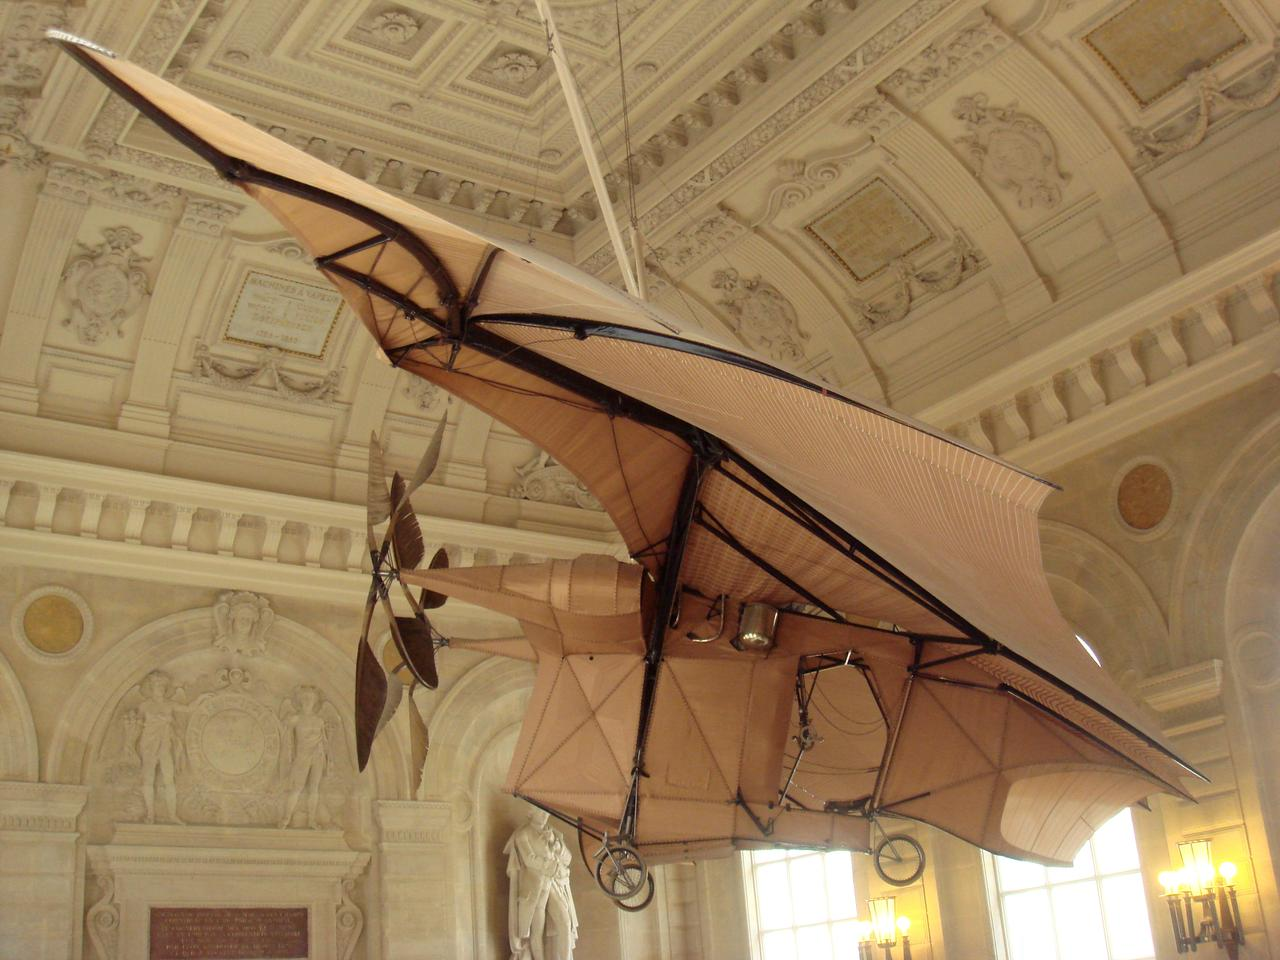
\includegraphics[width=1\linewidth]{Annexes/friseChronologique/img/Avion_III_Art_et_Metiers.jpg}
			\legende{L'Avion III de Clément Ader}{frise:Avion_III_Art_et_Metiers.jpg}
		\end{figure}	
		\end{column}
		\begin{column}{0.6\textwidth}
			La fin du \siecle{19} et le début du \siecle{20} sont marqués par une course effrénée vers le vol motorisé "plus lourd que l'air".	\newline
			
			En 1890, Clément Ader, ingénieur français, conçoit l'Eole puis les Avions, aérodynes en forme de chauves-souris. Bien que Clément Ader affirma à partir de 1906 que ses aérodynes soient parvenus à réaliser des vols de 300 m, on manque de preuve pour attester ces affirmations. Pour cette raison, on ne retient pas Ader comme ayant été le premier à effectuer un vol contrôlé.
		\end{column}
		\end{columns}
	\end{frame} 	
	
	\begin{frame}{Premiers pas des plus lourds que l'air}
	\begin{columns}
		\begin{column}{0.4\textwidth}
		\begin{figure}[H]
			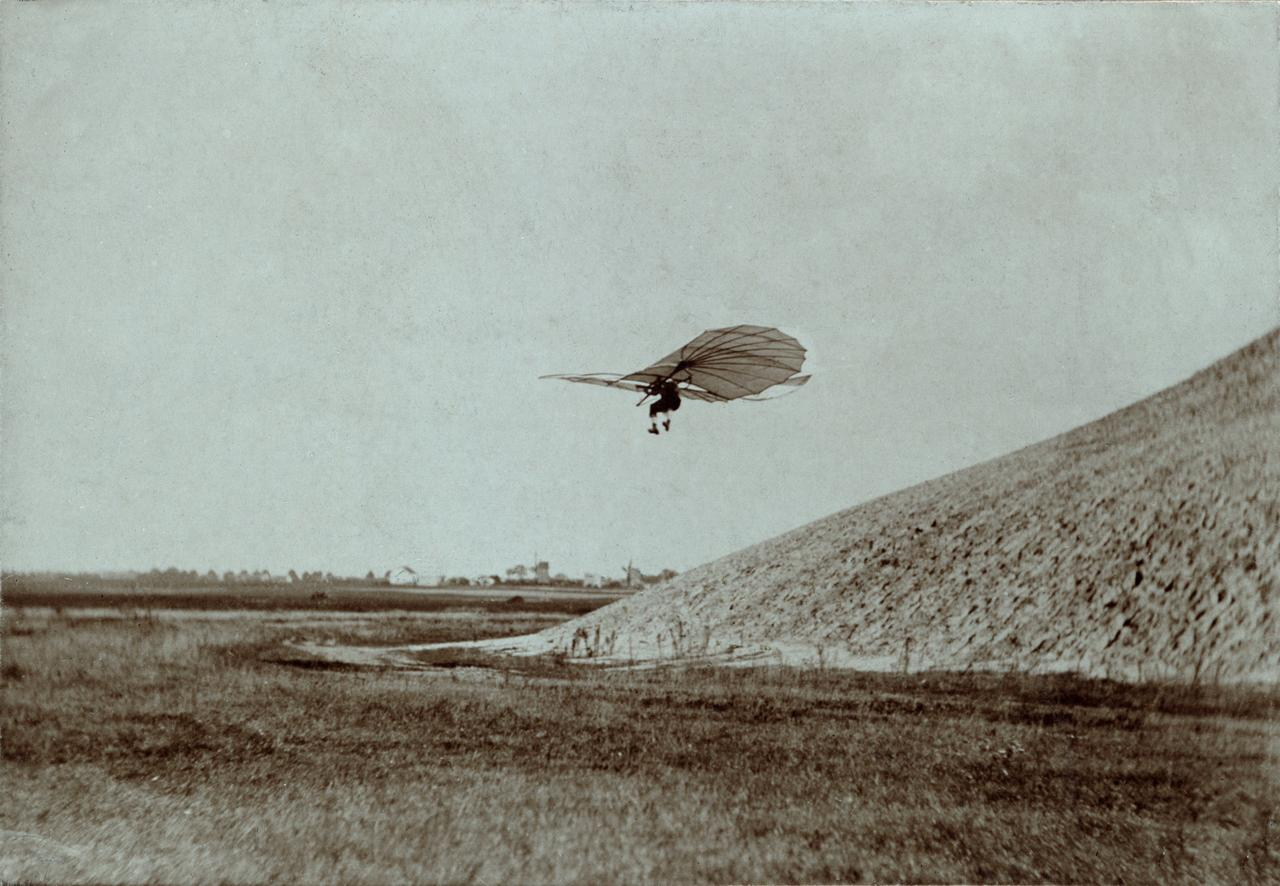
\includegraphics[width=1\linewidth]{Annexes/friseChronologique/img/Otto_Lilienthal_gliding_experiment_ppmsca.02546.jpg}
			\legende{Vol d'Otto Lilienthal en 1895}{frise:Otto_Lilienthal_gliding_experiment_ppmsca.02546.jpg}
		\end{figure}	
		\end{column}
		\begin{column}{0.6\textwidth}
			En 1891, l'ingénieur allemand Otto Lilienthal fait voler son planeur, en se lançant depuis une colline. Il devient ainsi le premier humain à évoluer dans les airs à bord d'un aéronef.
		\end{column}
		\end{columns}
	\end{frame} 	
	
	\begin{frame}{Premiers pas des plus lourds que l'air}
	\begin{columns}
		\begin{column}{0.4\textwidth}
		\begin{figure}[H]
			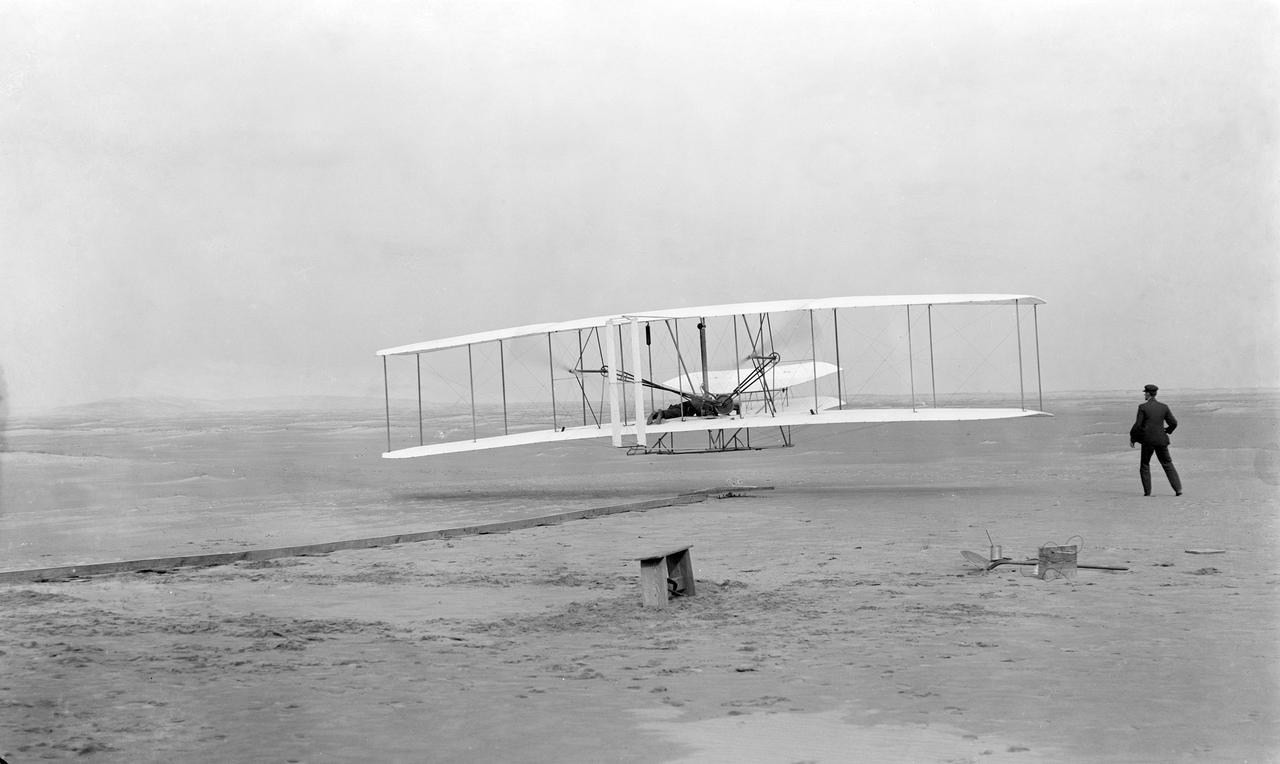
\includegraphics[width=1\linewidth]{Annexes/friseChronologique/img/Wrightflyer.jpg}
			\legende{Le Wright Flyer}{frise:Wrightflyer.jpg}
		\end{figure}	
		\end{column}
		\begin{column}{0.6\textwidth}
			En 1903, les frères Orville et Wilbur Wright font voler leur avion aux États-Unis.
Il s'agit du premier vol contrôlé d'un aérodyne motorisé.
		\end{column}
		\end{columns}
	\end{frame}
	
	\subsection{Les perfectionnements}
	\begin{frame}{Invention du manche à balai}
	\begin{columns}
		\begin{column}{0.4\textwidth}
		\begin{figure}[H]
			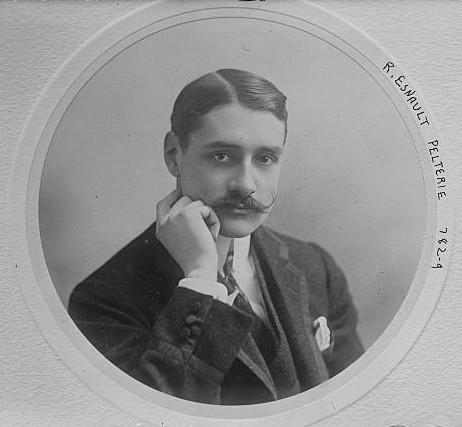
\includegraphics[width=1\linewidth]{Annexes/friseChronologique/img/Robert_Esnault-Pelterie_1909.jpg}
			\legende{Portrait de Robert Esnault-Pelterie}{frise:Robert_Esnault-Pelterie_1909.jpg}
		\end{figure}	
		\end{column}
		\begin{column}{0.6\textwidth}
			En 1907, l'ingénieur français Robert Esnault-Pelterie dépose le brevet pour le manche à balai, permettant de diriger les aéronefs
		\end{column}
		\end{columns}
	\end{frame}
	
	\begin{frame}{Premiers exploits : traversées maritimes}
	\begin{columns}
		\begin{column}{0.4\textwidth}
		\begin{figure}[H]
			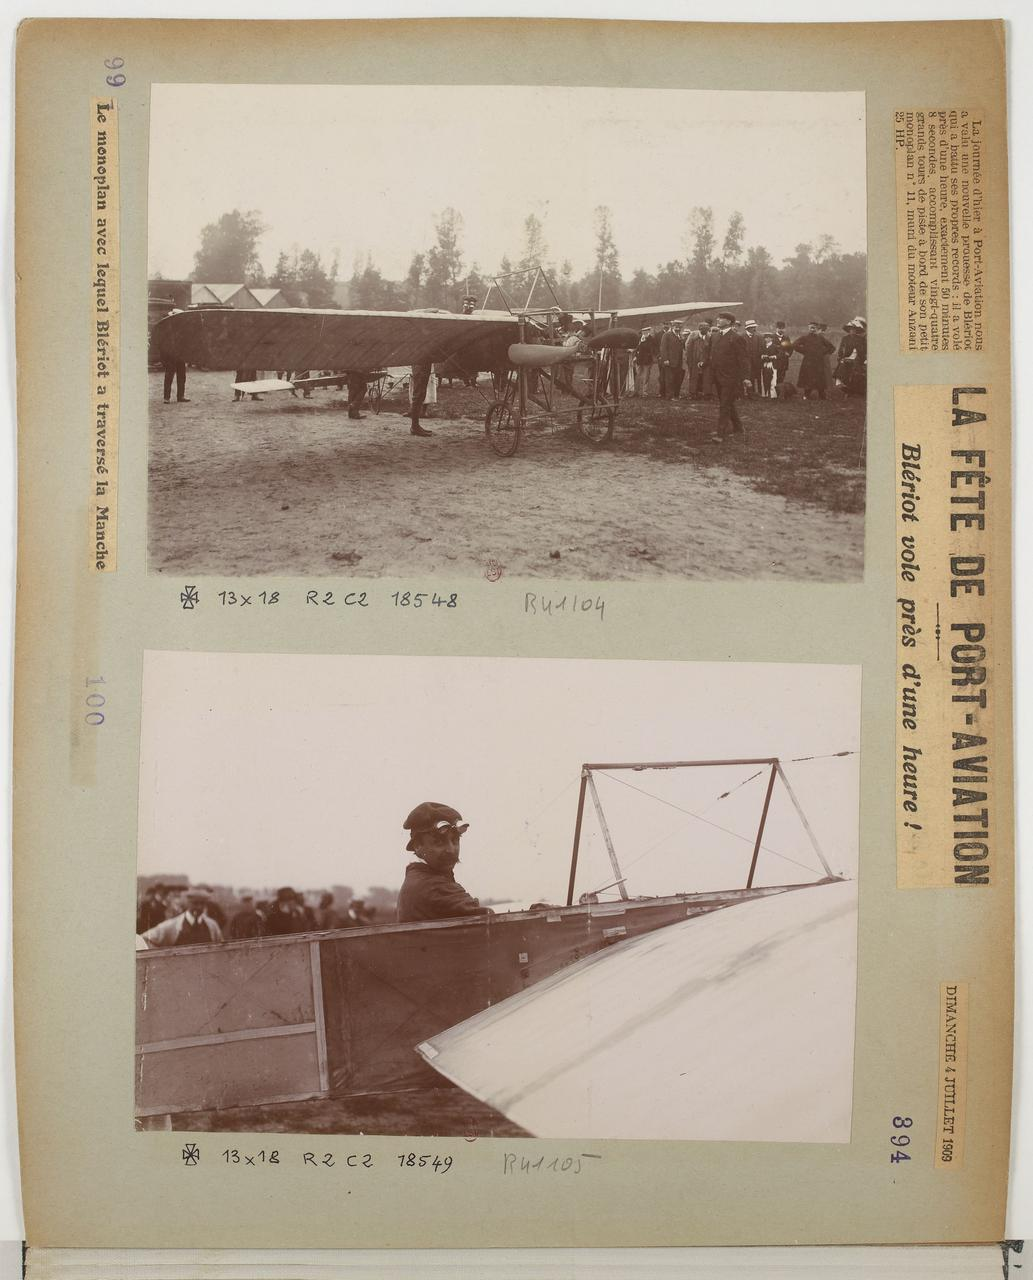
\includegraphics[width=0.8\linewidth]{Annexes/friseChronologique/img/Btv1b8433368f-p044_BlC3A9riot_C3A0_la_fC3AAte_de_Port-Aviation2C_dimanche_4_juillet_1909.jpg}
			\legende{Blériot aux commandes de l'appareil de la traversée à la fête de Port-Aviation, le 4 juillet 1909.}{frise:Btv1b8433368f-p044_BlC3A9riot_C3A0_la_fC3AAte_de_Port-Aviation2C_dimanche_4_juillet_1909}
		\end{figure}	
		\end{column}
		\begin{column}{0.6\textwidth}
			25 juillet 1909 : "L'Angleterre n'est plus une île !" Le 25 juillet 1909, Louis Blériot relie Calais à Douvres à bord de son  Blériot XI. \newline
			
			Le 7 octobre 1909, Louis Blériot se verra décerner le premier brevet de pilote du monde (brevet numéro 1, décerné par l'Aéroclub de France). \newline
			
			Le 8 mars 1910, Elisa Deroche se verra également attribuer un brevet de pilote : elle devient la première femme brevetée pilote au monde. \newline
		\end{column}
		\end{columns}
	\end{frame}
	
	\begin{frame}{Naissance de l'hydraviation}
	\begin{columns}
		\begin{column}{0.4\textwidth}
		\begin{figure}[H]
			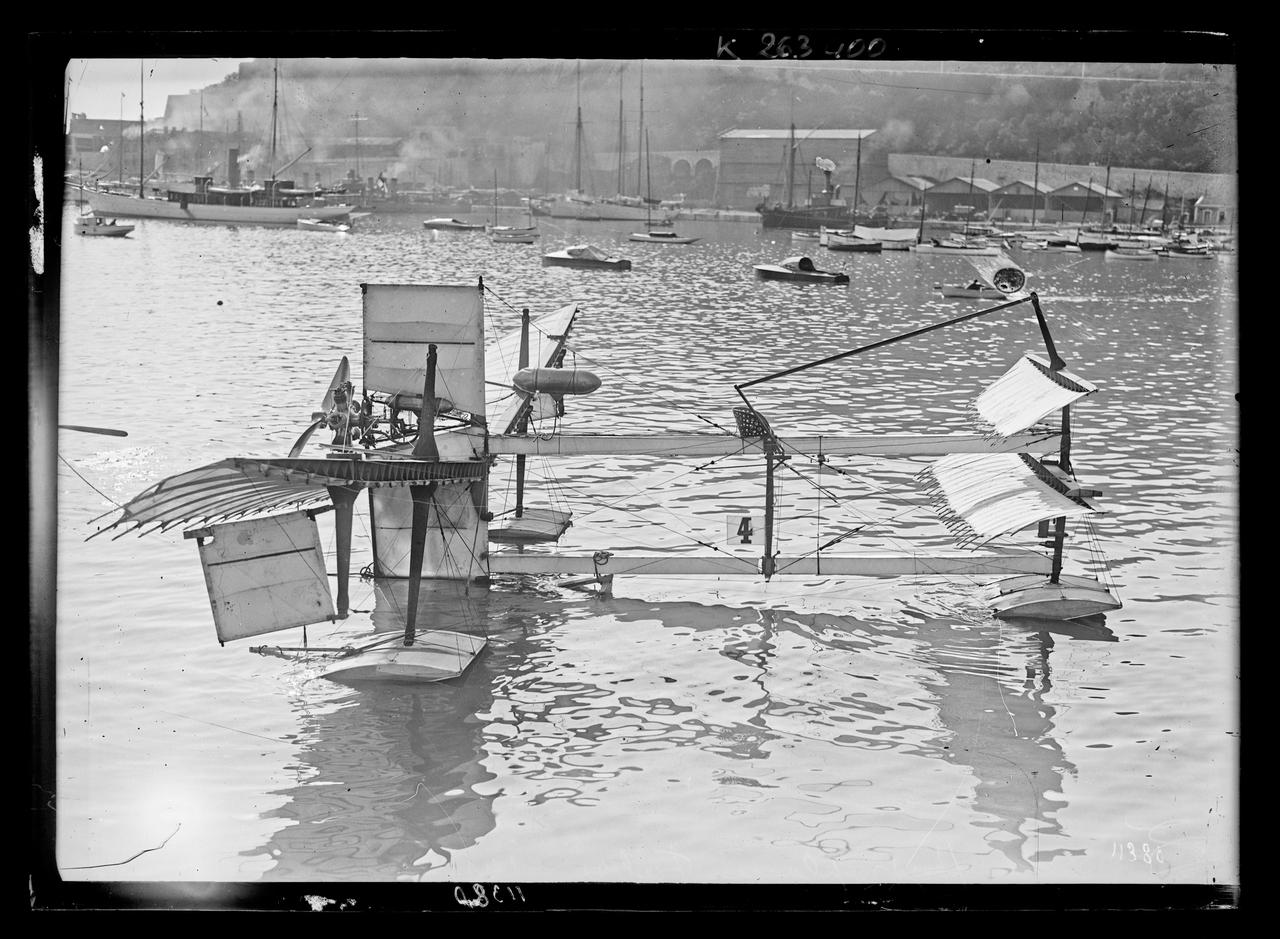
\includegraphics[width=1\linewidth]{Annexes/friseChronologique/img/Hydroplane_28de_Henri29_Fabre_28Monaco2C_concours_de_canots_automobiles2C_2_-17_avril29_1911_-_btv1b53240713d.jpg}
			\legende{L'hydroplane d'Henri Fabre}{frise:Hydroplane_28de_Henri29_Fabre_28Monaco2C_concours_de_canots_automobiles2C_2_-17_avril29_1911_-_btv1b53240713d}
		\end{figure}	
		\end{column}
		\begin{column}{0.6\textwidth}
			En 1910,  l'ingénieur français Henri Fabre devient le premier à décoller d'un plan d'eau avec un aéronef qui dispose de son propre moyen de propulsion. Cette date marque l'entrée dans l'ère de l'hydraviation qui aura par la suite son âge d'or sur la période de l'entre-deux-guerres.
		\end{column}
		\end{columns}
	\end{frame}
	
	\begin{frame}{Les aéronefs comme outil militaire}
	\begin{columns}
		\begin{column}{0.35\textwidth}
		\begin{figure}[H]
			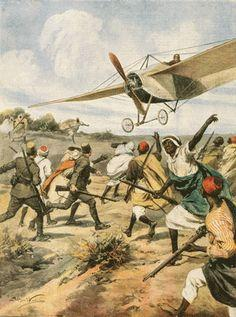
\includegraphics[width=0.9\linewidth]{Annexes/friseChronologique/img/Italian_Nieuport_IV_attacking_Ottoman_forces_in_Libya_1911_or_1912.jpg}
			\legende{Avion italien lors d'une attaque en Libye}{frise:Italian_Nieuport_IV_attacking_Ottoman_forces_in_Libya_1911_or_1912}
		\end{figure}	
		\end{column}
		\begin{column}{0.65\textwidth}
			En 1911, les Italiens sont les premiers à utiliser des avions au combat à l'occasion de la guerre de Libye. \newline
			
			Durant la première guerre mondiale, des ballons captifs sont utilisés pour l'observation : ils permettent de voir loin, et donc de rester à distance des armes ennemies. \newline
			
			La première guerre mondiale verra également la naissance du combat aérien, avec l'émergence de pilotes que l'on nommera les as : l'allemand Max Immelmann ou encore le français René Fonck, "l'as des as", qui sera crédité de 75 victoires et son concurrent allemand Manfred von Richtoffen (80).
		\end{column}
		\end{columns}
	\end{frame}
	
	\begin{frame}{L'hélice Éclair}
	\begin{columns}
		\begin{column}{0.4\textwidth}
		\begin{figure}[H]
			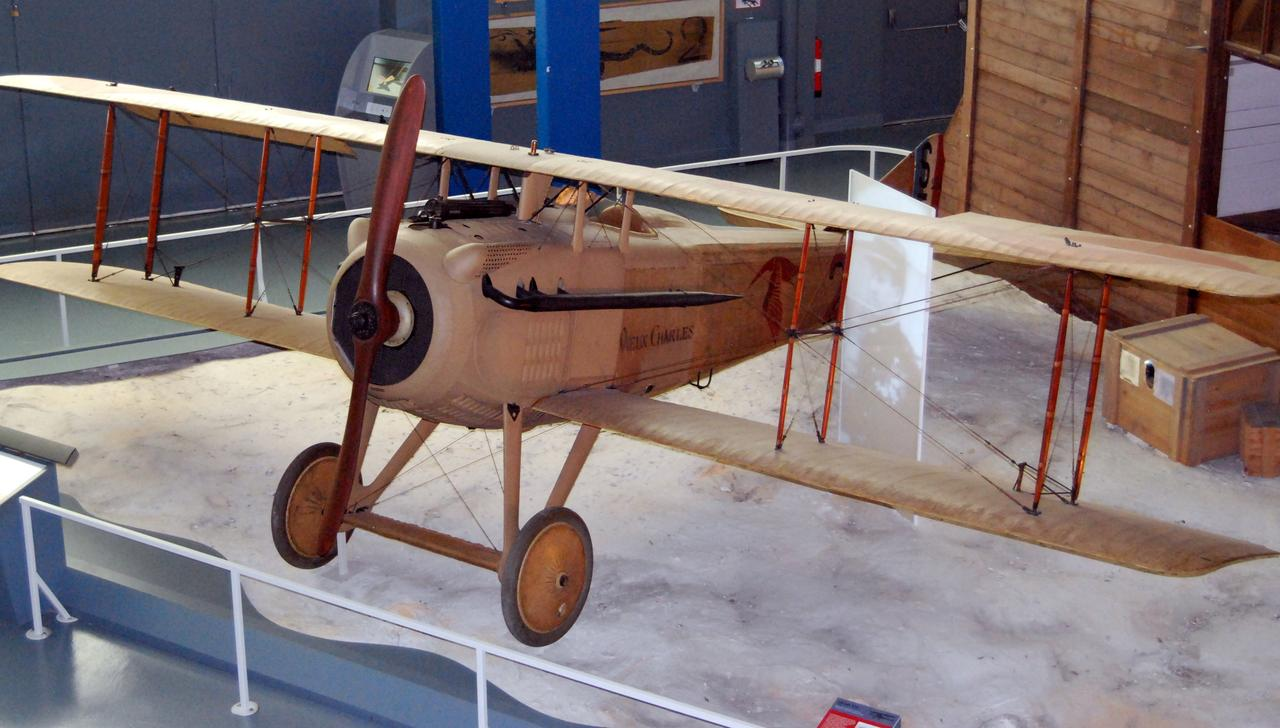
\includegraphics[width=1\linewidth]{Annexes/friseChronologique/img/Georges_Guynemer27s_SPAD_VII2C_Musee_de_l27Air_et_de_l27Espace2C_Le_Bourget2C_Paris._28812284872329.jpg}
			\legende{Le SPAD VII de Georges Guynemer, équipé de l'hélice Éclair}{frise:Georges_Guynemer27s_SPAD_VII2C_Musee_de_l27Air_et_de_l27Espace2C_Le_Bourget2C_Paris._28812284872329}
		\end{figure}	
		\end{column}
		\begin{column}{0.6\textwidth}
			En 1916, Marcel Dassault (qui s'appelait alors Marcel Bloch) dessine l'hélice Éclair. Cette hélice a marqué l'histoire car elle est très performante. Elle sera produite à plus de 4000 exemplaires et montée sur 10 des 20 avions les plus performants de l'armée française de cette époque.
		\end{column}
		\end{columns}
	\end{frame}
	
\appendix 
%\section{QCM}
%\qmcBia{Navigation, réglementation, sécurité des vols}
%{1}{Pour la sécurité des vols, la qualité qu'il faut avoir en priorité est :}
%{une bonne connaissance de soi, de ses limites et de sa machine}
%{une grande habileté de pilotage}
%{un grand nombre d'heures de pilotage}
%{une bonne connaissance de la réglementation} 
%{}



 
\input{commun/beamerSlidesBiblio.tex} 
 
\end{document}
